\documentclass[landscape]{article}
\usepackage{graphicx,amssymb,color}
\pagestyle{empty}
\oddsidemargin  -0.5 in
\evensidemargin -0.5 in
\headheight     0 in
\topmargin      -1 in
\textheight     7.7 in
\textwidth      10 in

\newcommand{\subs}[1]{{\mbox{\large #1}}}
\newcommand{\inv}{$^{-1}$}
\newcommand{\PM}{$\pm$}
\newcommand{\ups}{$\Upsilon$}
\newcommand{\gee}{{\boldmath $\Gamma_{ee}$}}
\newcommand{\us}{$\Upsilon(1S)$}
\newcommand{\uss}{$\Upsilon(2S)$}
\newcommand{\usss}{$\Upsilon(3S)$}
\newcommand{\es}{$\epsilon_{1S}$}
\newcommand{\ess}{$\epsilon_{2S}$}
\newcommand{\esss}{$\epsilon_{3S}$}
\newcommand{\ee}{$e^+e^-$}
\newcommand{\mumu}{$\mu^+\mu^-$}
\newcommand{\tautau}{$\tau^+\tau^-$}
\newcommand{\gamgam}{$\gamma\gamma$}
%\newcommand{\ggg}{$ggg$}
\newcommand{\gggamma}{$gg\gamma$}
\newcommand{\qqbar}{$q\bar{q}$}
\newcommand{\bee}{${\mathcal B}_{ee}$}
\newcommand{\bmm}{${\mathcal B}_{\mu\mu}$}
\newcommand{\btt}{${\mathcal B}_{\tau\tau}$}
\newcommand{\bcas}{${\mathcal B}_\subs{cas}$}
\newcommand{\geehadtot}{$\Gamma_{ee}\Gamma_\subs{had}/\Gamma_\subs{tot}$}
\newcommand{\twotoone}{$\Upsilon(2S) \to \pi^+\pi^- \Upsilon(1S)$}
\newcommand{\pipi}{$\pi^+\pi^-$}
\newcommand{\evis}{$\epsilon_\subs{vis}$}
\newcommand{\ecuts}{$\epsilon_\subs{cuts}$}
\newcommand{\ebeam}{$E_\subs{beam}$}
\newcommand{\ecm}{$E_\subs{CM}$}
\newcommand{\pmax}{$|\vec{p}_\subs{max}|$}
\newcommand{\visen}{$E_\subs{vis}$}
\newcommand{\dxy}{$d_\subs{XY}$}
\newcommand{\dz}{$d_\subs{Z}$}
\newcommand{\vtd}{$V_{td}$}
\newcommand{\twotrack}{{\tt two-track}}
\newcommand{\hadron}{{\tt hadron}}
\newcommand{\radtau}{{\tt rad-tau}}
\newcommand{\eltrack}{{\tt $e^\pm$-track}}
\newcommand{\barrelbhabha}{{\tt barrel-bhabha}}
\newcommand{\axial}{{\tt AXIAL}}
\newcommand{\stereo}{{\tt STEREO}}
\newcommand{\cblo}{{\tt CBLO}}
\newcommand{\cbmd}{{\tt CBMD}}
\newcommand{\cbhi}{{\tt CBHI}}
\definecolor{dkgreen}{rgb}{0.0,0.5,0.0}
\definecolor{dkgrey}{rgb}{0.3,0.3,0.3}

\begin{document}
\huge \sffamily
\renewcommand{\labelitemi}{{\LARGE $\stackrel{\bullet}{\mbox{ }}$}}
\setlength{\parindent}{0 cm}
\newenvironment{slide}{\begin{tabular}{l} {\color{black} intro} \hfill {\color{black} technique} \hfill {\color{black} backgrounds} \hfill {\color{black} efficiency} \hfill {\color{black} luminosity} \hfill {\color{black} energy} \hfill {\color{black} fitting} \hfill {\color{black} interference} \hfill {\color{black} conclusions} \\\hline\end{tabular} \vfill}{\vfill \mbox{ } \pagebreak}
\newenvironment{slide:intro}{\begin{tabular}{l} {\color{blue} intro} \hfill {\color{black} technique} \hfill {\color{black} backgrounds} \hfill {\color{black} efficiency} \hfill {\color{black} luminosity} \hfill {\color{black} energy} \hfill {\color{black} fitting} \hfill {\color{black} interference} \hfill {\color{black} conclusions} \\\hline\end{tabular} \vfill}{\vfill \mbox{ } \hfill \Large \arabic{page} \pagebreak}
\newenvironment{slide:technique}{\begin{tabular}{l} {\color{black} intro} \hfill {\color{blue} technique} \hfill {\color{black} backgrounds} \hfill {\color{black} efficiency} \hfill {\color{black} luminosity} \hfill {\color{black} energy} \hfill {\color{black} fitting} \hfill {\color{black} interference} \hfill {\color{black} conclusions} \\\hline\end{tabular} \vfill}{\vfill \mbox{ } \hfill \Large \arabic{page} \pagebreak}
\newenvironment{slide:backgrounds}{\begin{tabular}{l} {\color{black} intro} \hfill {\color{black} technique} \hfill {\color{blue} backgrounds} \hfill {\color{black} efficiency} \hfill {\color{black} luminosity} \hfill {\color{black} energy} \hfill {\color{black} fitting} \hfill {\color{black} interference} \hfill {\color{black} conclusions} \\\hline\end{tabular} \vfill}{\vfill \mbox{ } \hfill \Large \arabic{page} \pagebreak}
\newenvironment{slide:efficiency}{\begin{tabular}{l} {\color{black} intro} \hfill {\color{black} technique} \hfill {\color{black} backgrounds} \hfill {\color{blue} efficiency} \hfill {\color{black} luminosity} \hfill {\color{black} energy} \hfill {\color{black} fitting} \hfill {\color{black} interference} \hfill {\color{black} conclusions} \\\hline\end{tabular} \vfill}{\vfill \mbox{ } \hfill \Large \arabic{page} \pagebreak}
\newenvironment{slide:luminosity}{\begin{tabular}{l} {\color{black} intro} \hfill {\color{black} technique} \hfill {\color{black} backgrounds} \hfill {\color{black} efficiency} \hfill {\color{blue} luminosity} \hfill {\color{black} energy} \hfill {\color{black} fitting} \hfill {\color{black} interference} \hfill {\color{black} conclusions} \\\hline\end{tabular} \vfill}{\vfill \mbox{ } \hfill \Large \arabic{page} \pagebreak}
\newenvironment{slide:energy}{\begin{tabular}{l} {\color{black} intro} \hfill {\color{black} technique} \hfill {\color{black} backgrounds} \hfill {\color{black} efficiency} \hfill {\color{black} luminosity} \hfill {\color{blue} energy} \hfill {\color{black} fitting} \hfill {\color{black} interference} \hfill {\color{black} conclusions} \\\hline\end{tabular} \vfill}{\vfill \mbox{ } \hfill \Large \arabic{page} \pagebreak}
\newenvironment{slide:fitting}{\begin{tabular}{l} {\color{black} intro} \hfill {\color{black} technique} \hfill {\color{black} backgrounds} \hfill {\color{black} efficiency} \hfill {\color{black} luminosity} \hfill {\color{black} energy} \hfill {\color{blue} fitting} \hfill {\color{black} interference} \hfill {\color{black} conclusions} \\\hline\end{tabular} \vfill}{\vfill \mbox{ } \hfill \Large \arabic{page} \pagebreak}
\newenvironment{slide:interference}{\begin{tabular}{l} {\color{black} intro} \hfill {\color{black} technique} \hfill {\color{black} backgrounds} \hfill {\color{black} efficiency} \hfill {\color{black} luminosity} \hfill {\color{black} energy} \hfill {\color{black} fitting} \hfill {\color{blue} interference} \hfill {\color{black} conclusions} \\\hline\end{tabular} \vfill}{\vfill \mbox{ } \hfill \Large \arabic{page} \pagebreak}
\newenvironment{slide:conclusions}{\begin{tabular}{l} {\color{black} intro} \hfill {\color{black} technique} \hfill {\color{black} backgrounds} \hfill {\color{black} efficiency} \hfill {\color{black} luminosity} \hfill {\color{black} energy} \hfill {\color{black} fitting} \hfill {\color{black} interference} \hfill {\color{blue} conclusions} \\\hline\end{tabular} \vfill}{\vfill \mbox{ } \hfill \Large \arabic{page} \pagebreak}

\begin{slide}
\begin{center}
\Huge
  Di-electron Widths of the $\Upsilon$(1S), $\Upsilon$(2S), and $\Upsilon$(3S)

  \vspace{2 cm} Jim Pivarski
\end{center}
\end{slide}

\addtocounter{page}{-1}

\begin{slide:intro}

The 3.5 Fundamental Interactions
\renewcommand{\arraystretch}{1.25}
\begin{center}
{\color{dkgrey}
\begin{tabular}{l}
  \mbox{ } \\
  mediated by \\
  sources
\end{tabular}
\begin{tabular}{c | c | c | c}
  Electro- & -Weak & \color{black} Strong Nuclear & Gravity \\ \hline
  photon ($\gamma$) & $W^\pm$, $Z^0$ & \color{black} gluons ($g$) & curved space \\
  all charged particles & all known particles & \color{black} quarks, gluons & mass
\end{tabular}}
\end{center}

\vfill
\begin{center}
\begin{tabular}{p{0.5\linewidth} p{0.05\linewidth} p{0.35\linewidth}}
\begin{minipage}{\linewidth}
Strong Nuclear force:
\begin{itemize}

  \item quarks have {\color{red} red,} {\color{dkgreen} green,} or {\color{blue} blue} charges

  \item anti-quarks have anti-colors

  \item gluons have color/anti-color

\end{itemize}
\end{minipage} & &
\begin{minipage}{\linewidth}
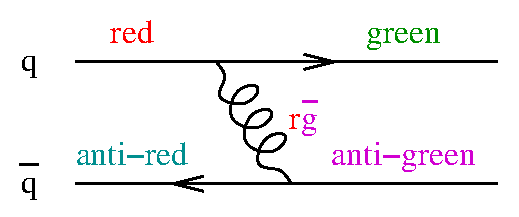
\includegraphics[width=\linewidth]{plots/intro1}
\end{minipage}
\end{tabular}
\end{center}

\vfill
This is the force that holds protons \mbox{\includegraphics[width=2.5 cm, viewport=0 49 157 146]{plots/intro2}}
and neutrons \mbox{\includegraphics[width=2.5 cm, viewport=0 49 157 146]{plots/intro3}} together.

\vfill
Fringe fields bind protons and neutrons into nuclei

\end{slide:intro}

\begin{slide:intro}

Color-charged gluons can self-interact: \hspace{0.5 cm} \mbox{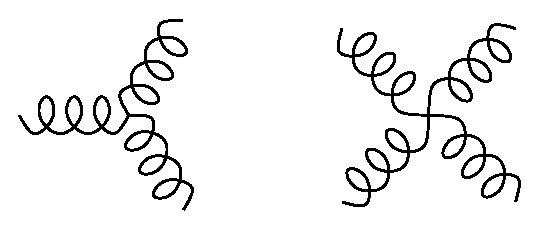
\includegraphics[width=6 cm, viewport=0 38 243 94]{plots/intro4}}

\vfill
\vspace{1 cm}
In Quantum Electrodynamics (QED), each graph contributes ${\mathcal O}(\alpha^N)$ to the amplitude
\[ \alpha = 1/137 \mbox{ and } N = \mbox{number of vertices in graph} \]

\vfill
In Quantum Chromodynamics (QCD) at large distances ($\gtrsim$ 0.2~fm = 1~GeV\inv),
\[ \alpha_s \sim 1 \]

\vfill
Complicated graphs cannot be ignored

\vspace{0.5 cm}
\begin{center}
\mbox{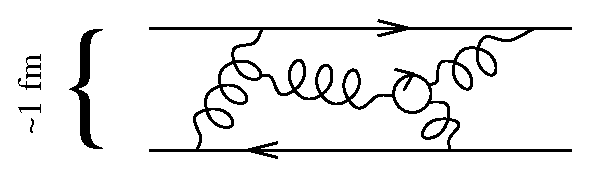
\includegraphics[height=1.2 cm, viewport=0 30 268 69]{plots/intro5}} \mbox{ }is not suppressed relative to\mbox{ } \mbox{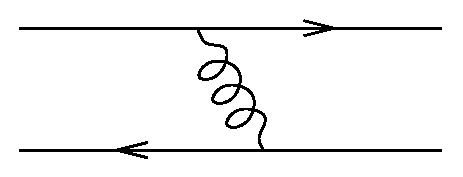
\includegraphics[height=1.2 cm, viewport=0 30 206 69]{plots/intro6}}
\end{center}

\vfill
\vspace{1 cm}
Large-distance QCD is very difficult to calculate

\end{slide:intro}

\begin{slide:intro}

Alternative method: Lattice QCD

\vfill
General problem is to compute amplitude = $\displaystyle \sum_f S[f]$
\begin{center}
\begin{tabular}{c l}
  $f$ & is a function of quark and gluon field values w.r.t.\ space-time \\
  $S$ & is the action (fundamental theory, in this case QCD)
\end{tabular}
\end{center}

\vfill
Rather than partitioning $\{f\}$ by topology, simulate random paths with a computer

\vfill
\begin{center}
\begin{tabular}{p{0.5\linewidth} p{0.45\linewidth}}
\begin{minipage}{\linewidth}
\begin{enumerate}\setlength{\itemsep}{0.75 cm}

  \item Discretize space-time

  \item Throw random paths $f$

  \item Interpolate with short-distance QCD

  \item Calculate $S(f)$ and integrate

  \item Take continuum limit from several simulations

\end{enumerate}
\end{minipage} &
\begin{minipage}{\linewidth}
\includegraphics[width=\linewidth]{plots/qcd_proton}
\end{minipage}
\end{tabular}
\end{center}

\end{slide:intro}

\begin{slide:intro}

Computationally intensive, particularly because of \includegraphics[width=6 cm, viewport=0 13 81 30]{thesis_newplots/vacuumpolarization}

\vfill
\vspace{1 cm}
Symanzik-improved staggered-quark formalism (1999) makes $u$, $d$, $s$ quark loops feasible

\vfill
\begin{center}
\includegraphics[width=0.6\linewidth]{thesis_plots/latticevictory}
\end{center}

\end{slide:intro}

\begin{slide:intro}
\begin{center}
\includegraphics[width=0.9\linewidth]{thesis_plots/fbresults}
\end{center}
\end{slide:intro}

\begin{slide:intro}

Di-electron width (\gee) of $\Upsilon(nS)$ is the rate of \hfill \includegraphics[width=0.43\linewidth, viewport=0 63 505 149]{plots/diagram_GeeU}

\vfill
\vspace{1 cm}
\gee\ can be calculated to high-precision using improved Lattice QCD

($\sim$10\% for \gee$(nS)$ and few percent for \gee$(nS)$/\gee$(mS)$)

\vfill
This calculation shares some aspects of $f_B$, and is an extremely non-relativistic test case

\vfill
\fbox{\begin{minipage}{\linewidth}
\begin{center}
\begin{minipage}{0.9\linewidth}
{\color{white} W}

We experimentally measured \gee\ for \us, \uss, and \usss

\begin{itemize}

  \item 50$\times$ largest previous \us\ dataset, many times more for \uss, \usss

  \item Total (statistical + systematic) uncertainties of 1.5\%, 1.8\%, and 1.8\%

  \item Three states in one study allow for significant uncertainty cancellation in ratios

\end{itemize}

{\color{white} W}
\end{minipage}
\end{center}
\end{minipage}}

\end{slide:intro}

\begin{slide:technique}

Determine $\Upsilon \to e^+e^-$ decay rate by measuring $e^+e^- \to \Upsilon$ cross-section

\vfill
\[ {\mathcal A}\left( \mbox{\includegraphics[width=0.35\linewidth, viewport=0 63 445 149]{plots/diagram_GeeU}} \right)
 = {\mathcal A}\left( \mbox{\includegraphics[width=0.35\linewidth, viewport=60 63 505 149]{plots/diagram_GeeU-reversed}} \right) \]

\vfill
{\Huge \[ \Gamma_{ee} = \frac{{M_\Upsilon}^2}{6\pi^2} \int \sigma(e^+e^- \to \Upsilon) \, dE \]}

\vfill

\begin{center}
\begin{tabular}{p{0.25\linewidth} p{0.05\linewidth} p{0.5\linewidth}}
\begin{minipage}{\linewidth}
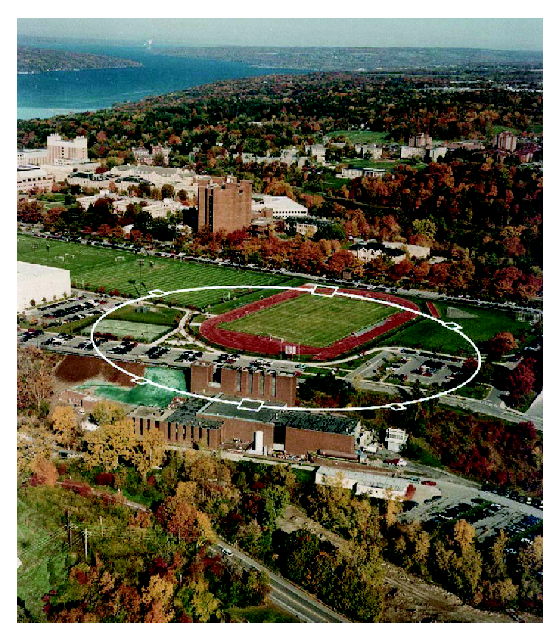
\includegraphics[width=\linewidth]{plots/aerial_200dpi}
\end{minipage} & &
\begin{minipage}{\linewidth}
\begin{enumerate}

  \item Collide $e^+$ and $e^-$ at different energies $E$

  \item Measure cross-section $\sigma(e^+e^- \to \Upsilon)$

  \item Integrate!

\end{enumerate}
\end{minipage}
\end{tabular}
\end{center}

\end{slide:technique}

\begin{slide:technique}
\begin{center}
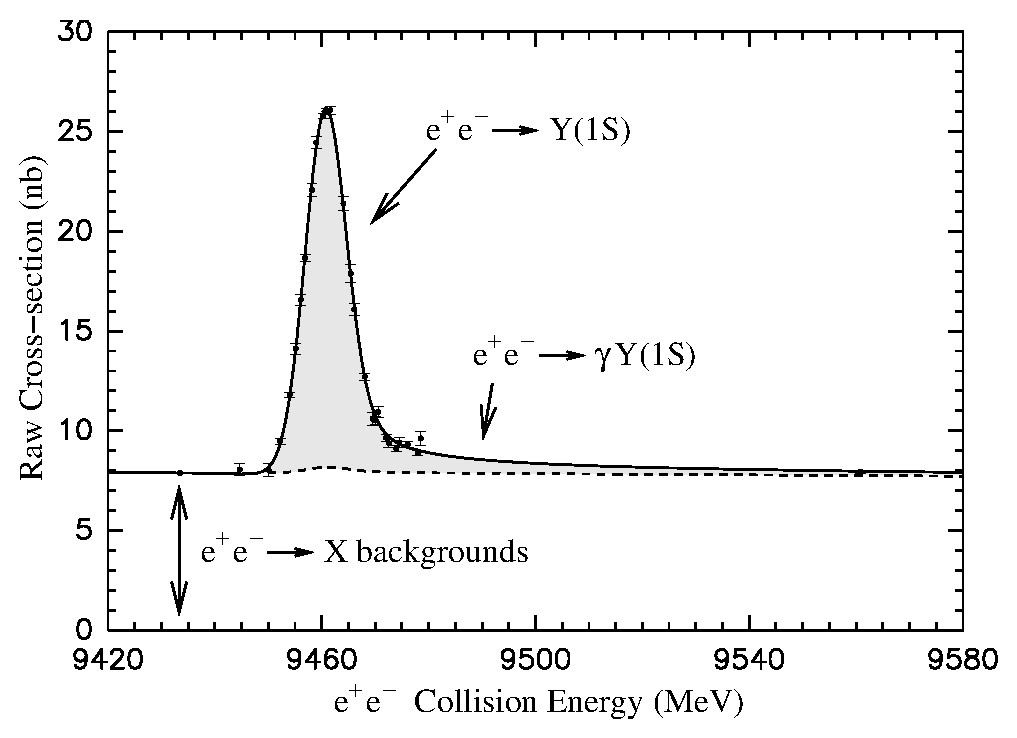
\includegraphics[width=0.9\linewidth]{plots/samplescan}
\end{center}
\end{slide:technique}

\begin{slide:technique}

\begin{center}
\begin{tabular}{p{0.3\linewidth} p{0.65\linewidth}}
\begin{minipage}{1.01\linewidth}

To measure $\sigma(e^+e^- \to \Upsilon)$,
\begin{center}
count \ups\ events
\end{center}

\begin{eqnarray*}
\sigma &=& \frac{N_\subs{obs} - N_\subs{back}}{\epsilon \, {\mathcal L}} \\
& & \\
N_\subs{obs} &=& \mbox{count} \\
N_\subs{back} &=& \mbox{backgrounds} \\
\epsilon &=& \mbox{efficiency} \\
{\mathcal L} &=& \mbox{luminosity}
\end{eqnarray*}

\end{minipage} &
\begin{minipage}{\linewidth}
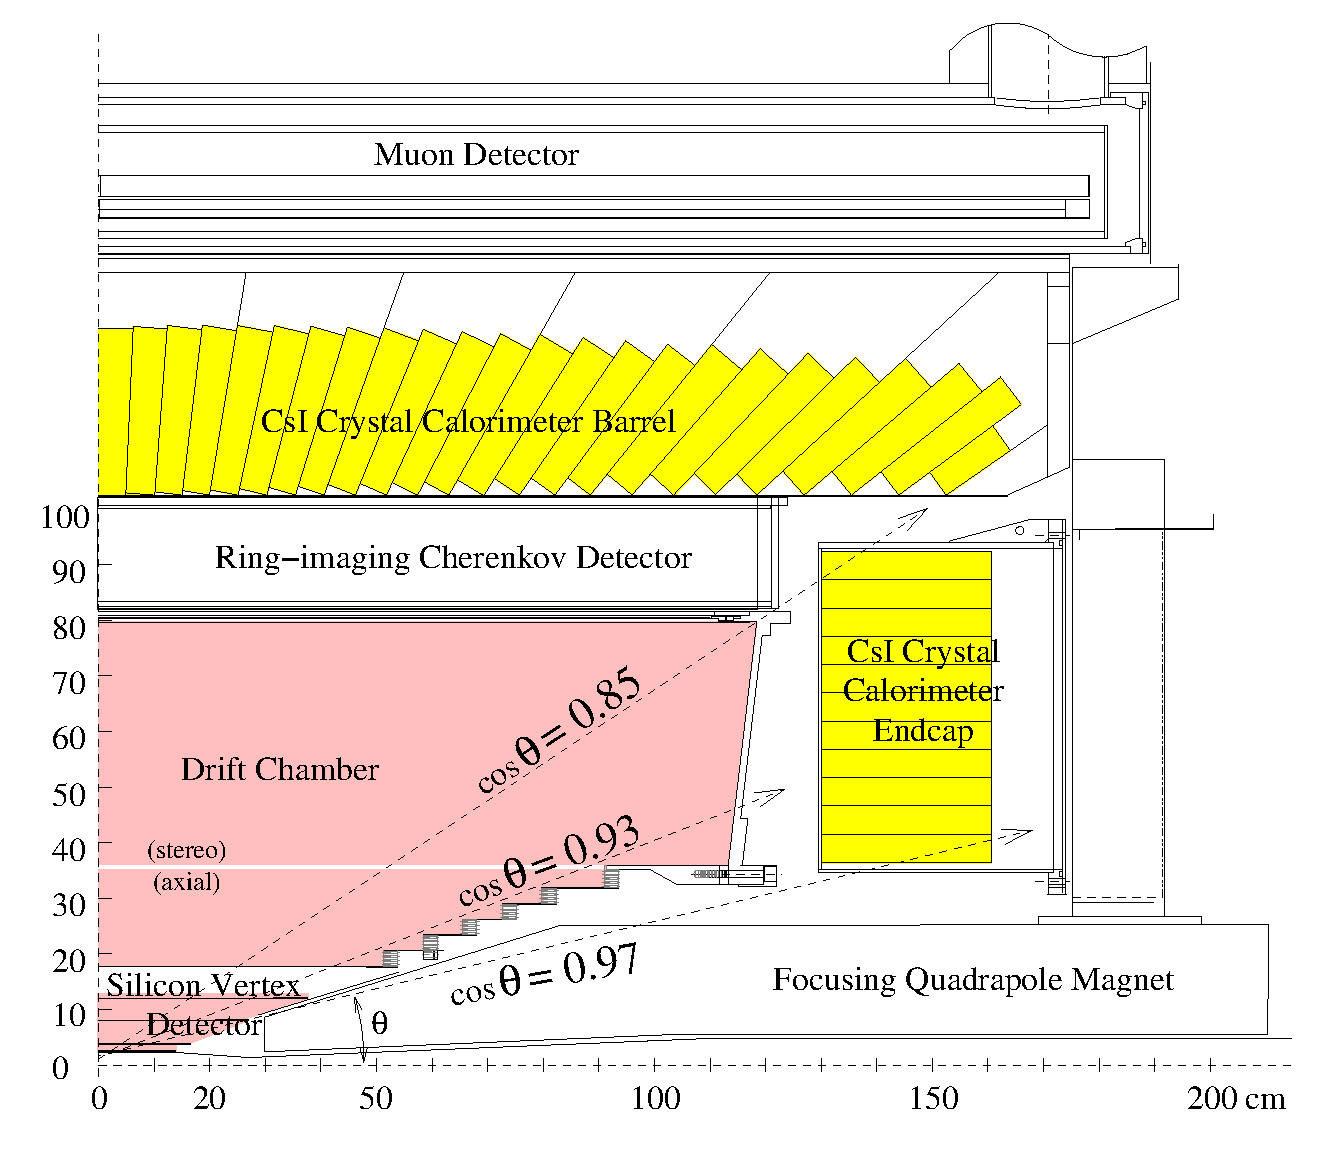
\includegraphics[width=\linewidth]{plots/quarterview}
\end{minipage}
\end{tabular}
\end{center}

\end{slide:technique}

\begin{slide:technique}

\begin{tabular}{l}
\ups\ decay modes \\\hline
\end{tabular}

\begin{itemize}

  \item leptonic: total of $3{\mathcal B}_{\mu\mu}$ = 7.5\%, well-measured

  \begin{itemize}

    \item \ee, \mumu, \tautau: hard to distinguish from background, easy to simulate

  \end{itemize}

  \item hadronic: total of $1 - 3{\mathcal B}_{\mu\mu}$, hard to simulate

  \begin{itemize}\setlength{\itemsep}{0.25 cm}

    \item $ggg$, $gg\gamma$, $q\bar{q} \to$ lots of particles

    \item \uss\ and \usss\ decay into lower-energy $b\bar{b}$ states, e.g.\ \twotoone

    \item unknown modes?

  \end{itemize}

\end{itemize}

\vfill
\begin{tabular}{l}
backgrounds \\\hline
\end{tabular}

\begin{itemize}

  \item $e^+e^- \to X$

  \begin{itemize}\setlength{\itemsep}{0.25 cm}

    \item \ee, \mumu, \tautau, \qqbar

    \item two-photon fusion: $e^+e^- \to e^+e^- X$

    \item $e^+e^- \to \gamma \Upsilon((n-1)S)$

  \end{itemize}

  \item beam-gas, beam-wall

  \item cosmic rays

\end{itemize}

\vspace{-1.5 cm}

\end{slide:technique}

\begin{slide:technique}

Select {\it hadronic} \ups\ decays, later correct with $(1 - 3{\mathcal B}_{\mu\mu})$

\vfill
\begin{center}
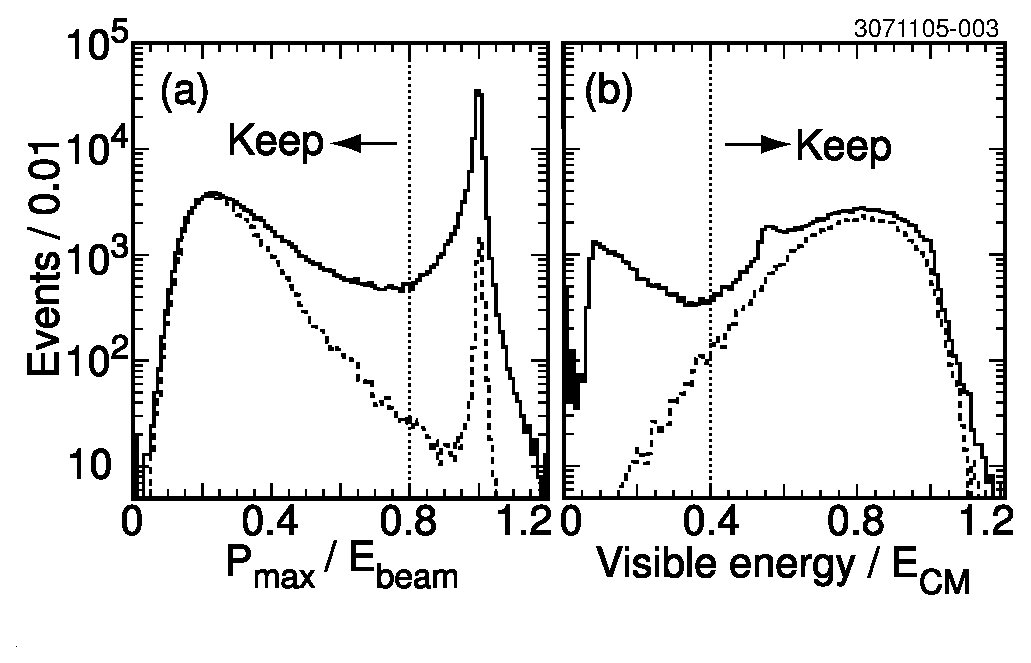
\includegraphics[width=0.8\linewidth]{plots/cuts}
\end{center}

\vspace{-1 cm}
solid are data

dashed are simulated \ups\ decays

all cuts applied except the one shown

\end{slide:technique}

\begin{slide:technique}

Select events near collision point ($<$ 7.5~cm along beam axis, $<$ 5~mm perpendicular)

\vfill
\begin{center}
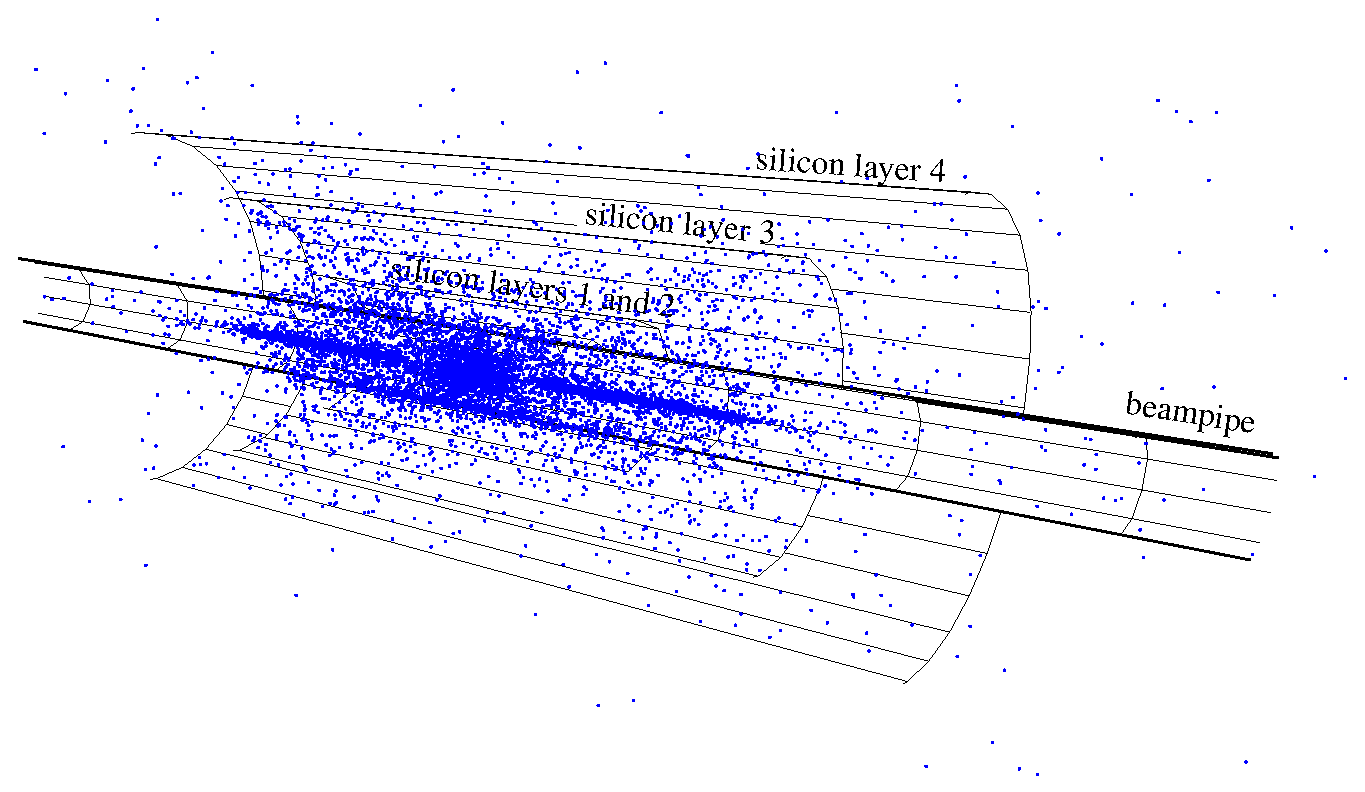
\includegraphics[width=0.8\linewidth]{plots/snazzy3d}
\end{center}

blue points are event vertices (determined from track intersections)

beam-beam collision region is suppressed

\end{slide:technique}

\begin{slide:backgrounds}
\begin{center}
\includegraphics[width=0.9\linewidth]{plots/awesome}
\end{center}
\vspace{-1 cm}
\end{slide:backgrounds}

\begin{slide:backgrounds}

Subtracting Cosmic Rays

\vfill
\begin{center}
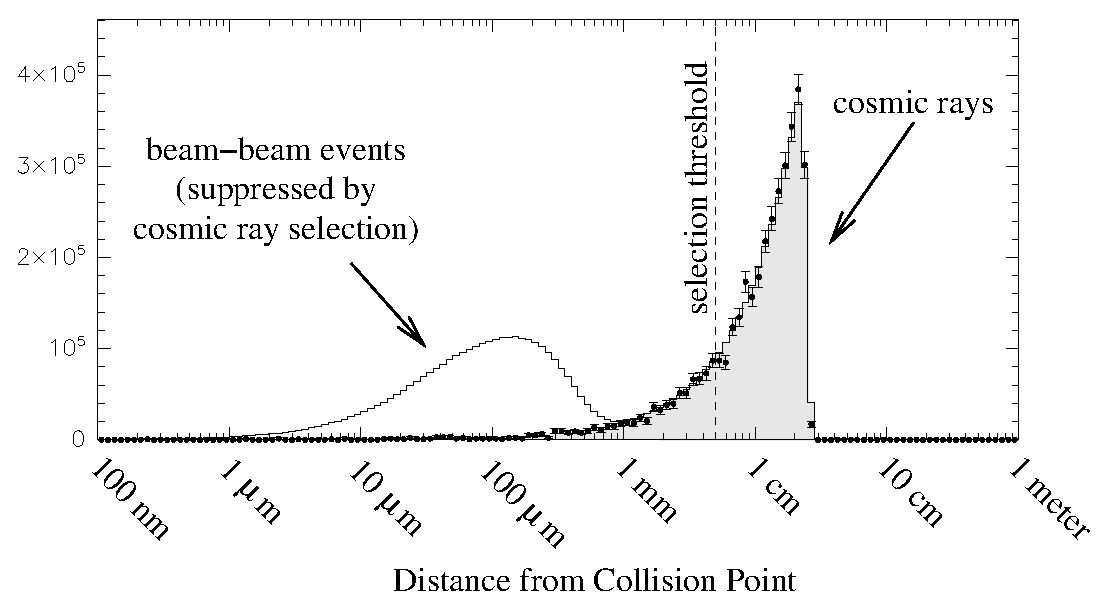
\includegraphics[width=0.9\linewidth]{plots/cosmicscontamination}
\end{center}

\vfill
solid histogram are beam-beam data

points with errorbars are no-beam data

\end{slide:backgrounds}

\begin{slide:efficiency}

Efficiency: what fraction of hadronic \ups\ decays are {\it missing} from our count?

\vfill
Hadronic modes are difficult to simulate, and our definition includes unknown modes

\vfill
\begin{tabular}{p{0.62\linewidth} c p{0.35\linewidth}}
  \begin{minipage}{\linewidth}
    \begin{itemize}\setlength{\itemsep}{0.75 cm}

      \item We have a large sample (1.3 fb\inv) of \uss\ decays

      \item Select \mbox{$\Upsilon(2S) \to \pi^+ \pi^- \ \Upsilon(1S)$} by $\pi^+ \pi^-$ recoil mass

        \begin{center}
          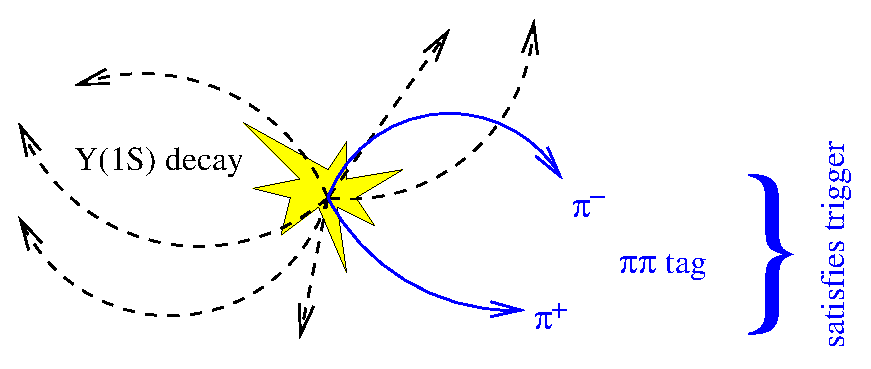
\includegraphics[width=0.9\linewidth]{plots/twotoone}
        \end{center}

      \item Set of $\Upsilon(1S)$ events is unbiased, includes all decays

      \item \us\ efficiency = \#pass/\#total = (97.8 $\pm$ 0.5)\%

    \end{itemize}
  \end{minipage} & & \begin{minipage}{\linewidth}
    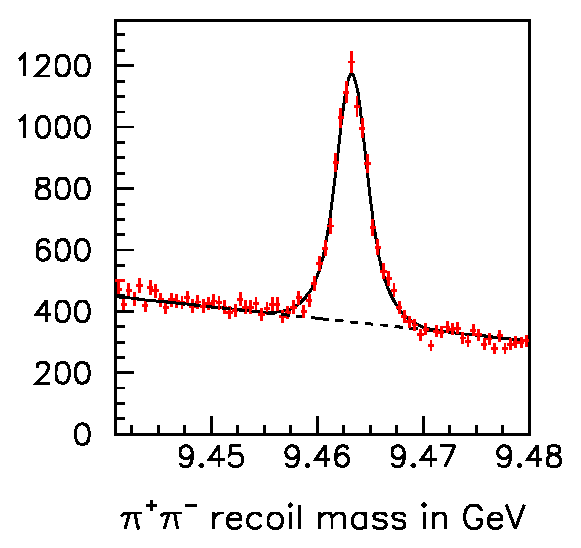
\includegraphics[width=\linewidth]{plots/pipimass}
  \end{minipage}
\end{tabular}

\end{slide:efficiency}

\begin{slide:efficiency}

Technical detail: \twotrack\ trigger satisfied by \pipi\ is prescaled by a factor of 19

\vfill
To get a statistically-precise result, we divide problem into two parts:

\begin{itemize}

  \item define \us\ decay to be visible if it generates one \axial\
  track and maybe one \cblo\ cluster in the trigger (the \cblo\ may be
  due to \pipi)

  \item define \evis\ = probability that \us\ is visible

  \item define \ecuts\ = probability that a visible \us\ decay passes cuts

\end{itemize}

\vspace{0.25 cm}
\begin{center}
\begin{tabular}{p{0.45\linewidth} p{0.45\linewidth}}
\begin{minipage}{\linewidth}
\begin{center}
determine \evis\ with a fit yield \\
from \twotrack\ trigger
\end{center}
\end{minipage} & 
\begin{minipage}{\linewidth}
\begin{center}
determine \ecuts\ with a background-subtracted count \\
from \hadron\ trigger
\end{center}
\end{minipage}
\end{tabular}

\vspace{0.5 cm}
\begin{tabular}{p{0.45\linewidth} p{0.45\linewidth}}
\begin{minipage}{\linewidth}
\includegraphics[width=\linewidth]{thesis_newplots/pipitwotrack}
\end{minipage} &
\begin{minipage}{\linewidth}
\includegraphics[width=\linewidth]{thesis_plots/pipihadron}
\end{minipage}
\end{tabular}
\end{center}

\end{slide:efficiency}

\begin{slide:efficiency}

Our efficiency study only applies to \us

\vfill
For \uss\ and \usss, we extrapolate using Monte Carlo simulations

\vfill
We assume that \uss\ and \usss\ decay like \us, but at higher energy
and with transitions to lower $b\bar{b}$ states

\vfill
\begin{center}
\begin{tabular}{p{0.25\linewidth} p{0.7\linewidth}}
\begin{minipage}{\linewidth}
Primary efficiency

correction:

\vspace{1 cm}
\includegraphics[width=\linewidth]{plots/cascadepic}

\vspace{1 cm}
$\Upsilon(nS) \to X\mu^+\mu^-$

\vspace{3.5 cm}

\end{minipage} &
\begin{minipage}{\linewidth}
\begin{center}
  Measuring ${\mathcal B}_{X\mu\mu}$ relative to ${\mathcal B}_{\mu\mu}$
\end{center}
\includegraphics[width=\linewidth]{thesis_plots/invariantmumass}

solid is Monte Carlo, shaded is $\mu^+\mu^-$, open is $X\mu^+\mu^-$

points with errorbars are data

\end{minipage}
\end{tabular}
\end{center}
\vspace{-1 cm}

\end{slide:efficiency}

\begin{slide:luminosity}

Reminder: cross-section $\displaystyle \sigma = (N_\subs{obs} - N_\subs{back})/(\epsilon \, {\mathcal L})$ where ${\mathcal L}$ is time-integrated luminosity

\vfill
Instantaneous luminosity is the intensity and degree of overlap of \ee\ beams

\vfill
Instantaneous luminosity is hard to measure and fluctuates with beam conditions

\vfill
Apply above equation for a process with a known cross-section

\vfill
$\sigma(e^+e^- \to e^+e^-) \times \epsilon(e^+e^-)$ may be calculated from QED and detector simulations

\vfill
\begin{center}
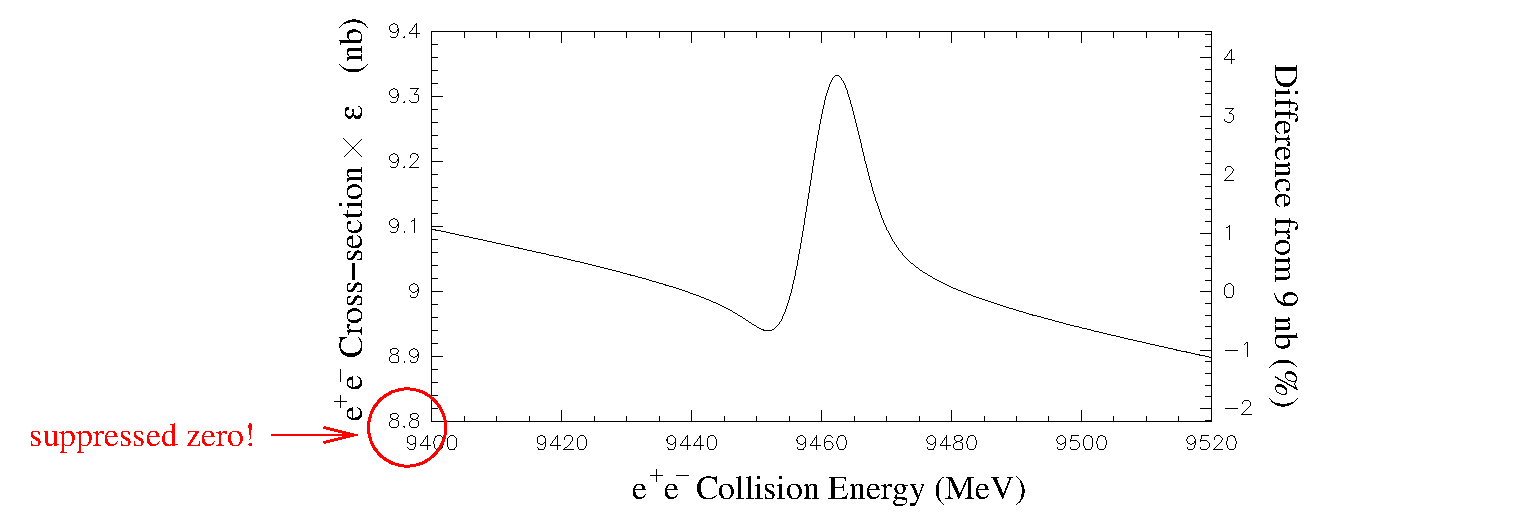
\includegraphics[width=0.9\linewidth]{plots/allee}
\end{center}

\vspace{-2 cm}
\end{slide:luminosity}

\begin{slide:luminosity}

Measure integrated luminosity three ways, consistent overall scale

\vfill
\begin{center}
\includegraphics[width=0.9\linewidth]{thesis_plots/comparelumis}
\end{center}

\end{slide:luminosity}

\begin{slide:luminosity}

BUT, we observe a difference in $e^+e^- \to \gamma\gamma$ as a function of \ee\ energy

\vfill
Unexplained: add to systematic uncertainty

\vfill
\begin{center}
\includegraphics[width=0.8\linewidth]{thesis_newplots/lumigamgam}
\end{center}

\vspace{-1 cm}
\end{slide:luminosity}

\begin{slide:energy}

\begin{center}
\begin{tabular}{p{0.6\linewidth} p{0.4\linewidth}}
\begin{minipage}{\linewidth}
So far, we have only considered vertical uncertainties

(uncertainties in cross-section)

\vspace{1 cm}
Now we turn to the horizontal: beam energy
\end{minipage} &
\begin{minipage}{\linewidth}
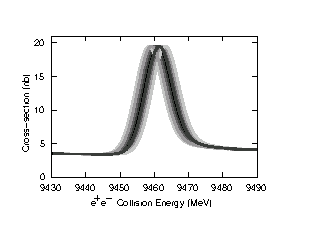
\includegraphics[width=\linewidth]{plots/energyuncertainty}
\end{minipage}
\end{tabular}
\end{center}

\vfill
Beam energy is determined by magnetic field measurements in storage ring magnets

\vfill
\[ E_\subs{beam} = \mbox{electron charge} \times \mbox{magnetic field} \times \mbox{storage ring radius} \]

\vfill
With corrections for

\vfill
\begin{center}
\begin{minipage}{0.95\linewidth}
\begin{itemize}

  \item RF frequency shifts

  \item steering and focusing magnets

  \item electrostatic separators

\end{itemize}
\end{minipage}
\end{center}

\vfill
Magnetic field probe is subject to shifts: \ebeam\ calibration may shift

\end{slide:energy}

\begin{slide:energy}

$M_\Upsilon$ is known: use \ups\ peaks as calibrating markers in beam energy

\vfill
\begin{center}
Repeated measurements of \us\ mass

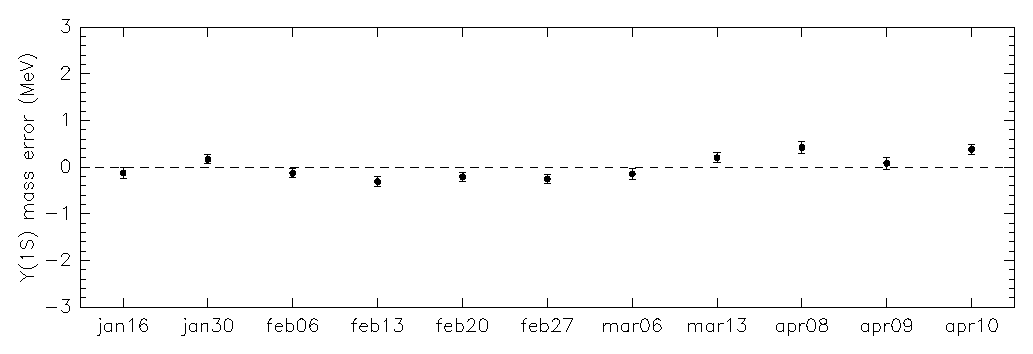
\includegraphics[width=\linewidth]{plots/beamenergydrift}
\end{center}

\vfill
\ee\ energy measurement drifts about 0.5~MeV/month

\vfill
We limit acceptable scan data to 48-hour windows

\end{slide:energy}

\begin{slide:energy}

\begin{tabular}{p{0.6\linewidth} p{0.38\linewidth}}
  \begin{minipage}{\linewidth}
    \begin{minipage}{0.9\linewidth}
      \begin{itemize}\setlength{\itemsep}{0.75 cm}

        \item Measurements alternated above and below resonance peak

        \item Point of high slope repeated ({\color{red} 1 \& 5}):
        convert cross-section reproducibility into beam energy reproducibility

        \end{itemize}

      \vspace{0.5 cm}
      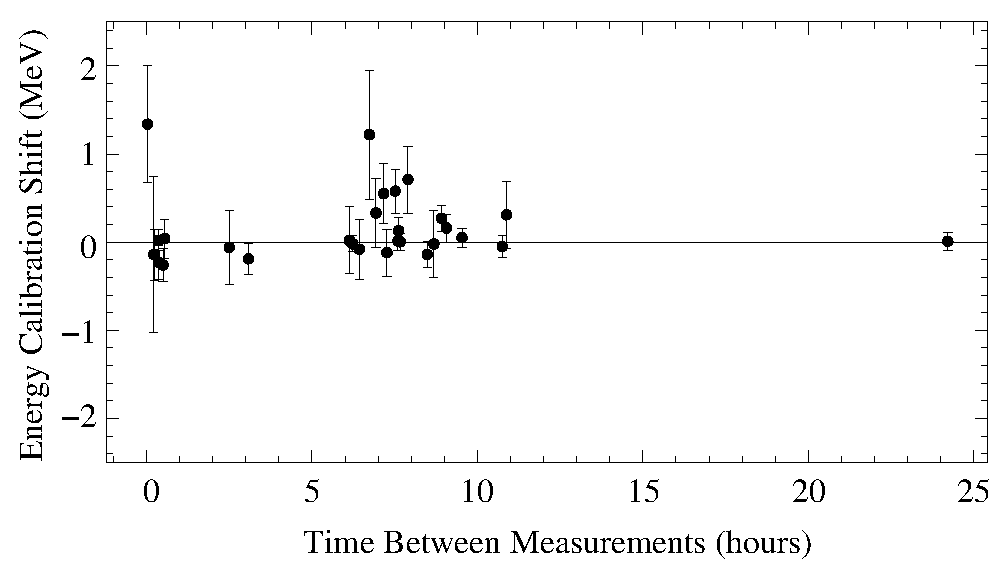
\includegraphics[width=\linewidth]{plots/miscalhours}

      \begin{itemize}\setlength{\itemsep}{0.75 cm}

        \item $\Rightarrow$ 0.07~MeV uncertainty in \ee\ energy,
	  \begin{center}
	    0.2\% in \gee
	  \end{center}

      \end{itemize}

    \end{minipage}

  \end{minipage} &
  \begin{minipage}{\linewidth}
    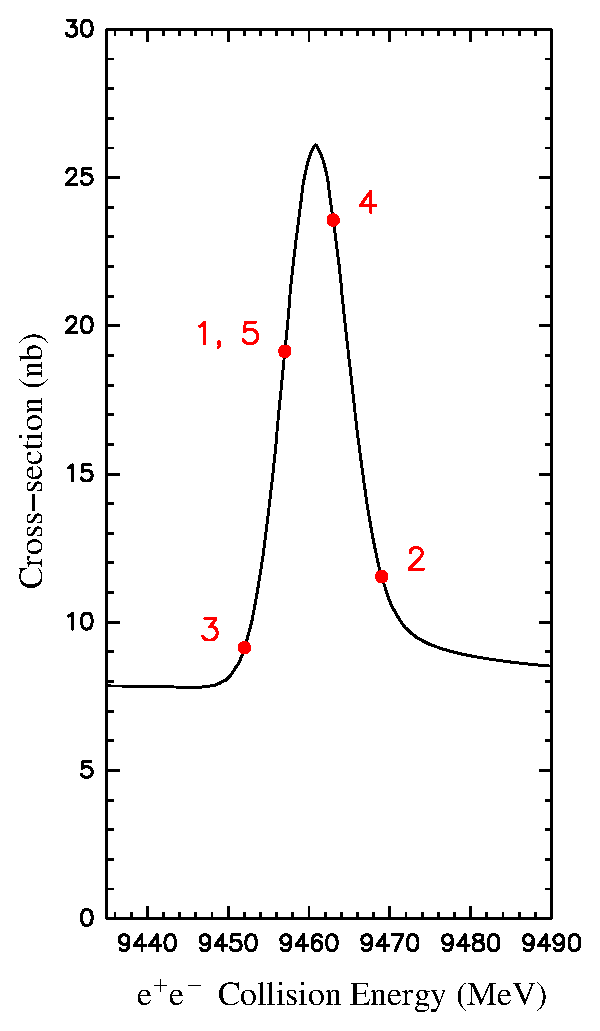
\includegraphics[width=\linewidth]{plots/fitorder}
  \end{minipage}
\end{tabular}

\end{slide:energy}

\begin{slide:fitting}

\begin{center}

{\Large \boldmath
\hspace{0.5 cm} \begin{tabular}{c c c}
  $\chi^2/N_\subs{dof} = 1.3$ \mbox{\hspace{4.2 cm}} & $\chi^2/N_\subs{dof} = 1.6$ & \mbox{\hspace{4.2 cm}} $\chi^2/N_\subs{dof} = 1.0$
\end{tabular}}
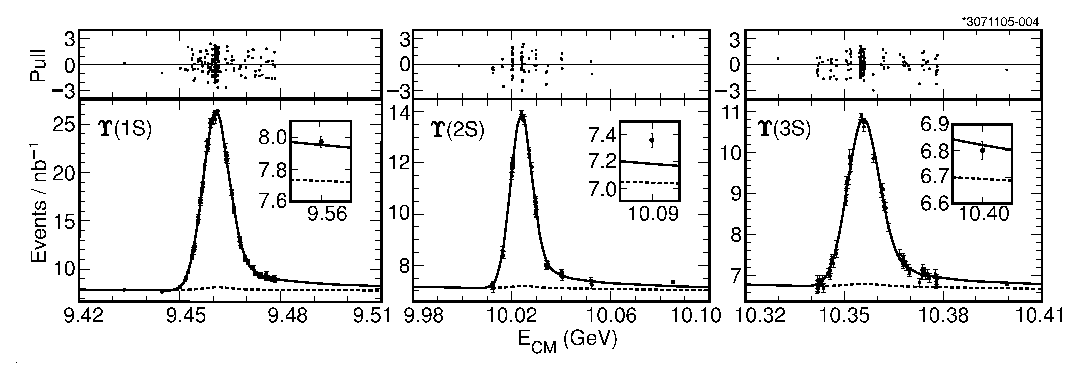
\includegraphics[width=\linewidth]{plots/fits}

\vfill
\renewcommand{\arraystretch}{1.2}
\begin{tabular}{c c c c c}
  & & & Statistical & Systematic \\
  \boldmath $\Gamma_{ee}(1S)$ & \mbox{\hspace{0.25 cm}} = \mbox{\hspace{0.25 cm}} & 1.354 $\pm$ 0.004 $\pm$ 0.020 keV & 0.3\% & 1.5\% \\
  & & & \\
  \boldmath $\Gamma_{ee}(2S)$ & = & 0.619 $\pm$ 0.004 $\pm$ 0.010 keV & 0.7\% & 1.6\% \\
  & & & \\
  \boldmath $\Gamma_{ee}(3S)$ & = & 0.446 $\pm$ $\underbrace{\mbox{0.004}}_{\mbox{stat}}$ $\pm$ $\underbrace{\mbox{0.007}}_{\mbox{syst}}$ keV & 1.0\% & 1.5\%
\end{tabular}

\end{center}

\end{slide:fitting}

\begin{slide:fitting}

\begin{center}
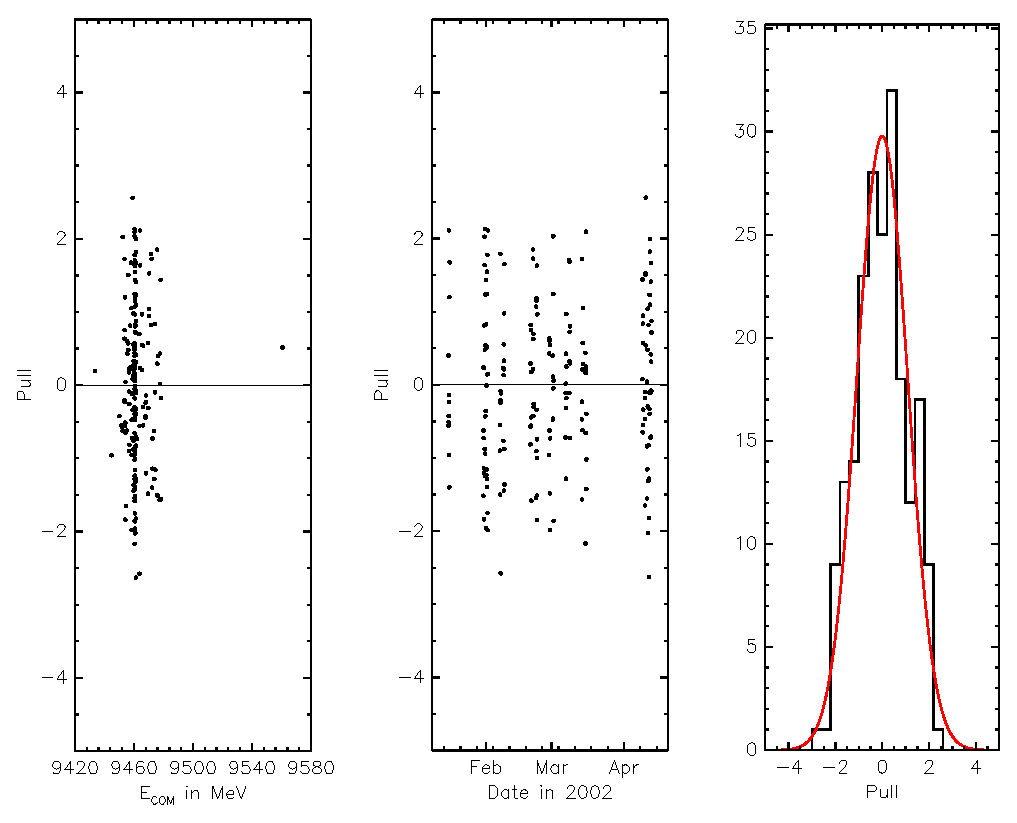
\includegraphics[width=0.8\linewidth]{plots/pulls1}
\end{center}

$\chi^2/N_\subs{dof}$ = 240/187 = 1.3, confidence level = 0.5\%

\end{slide:fitting}

\begin{slide:fitting}

\begin{center}
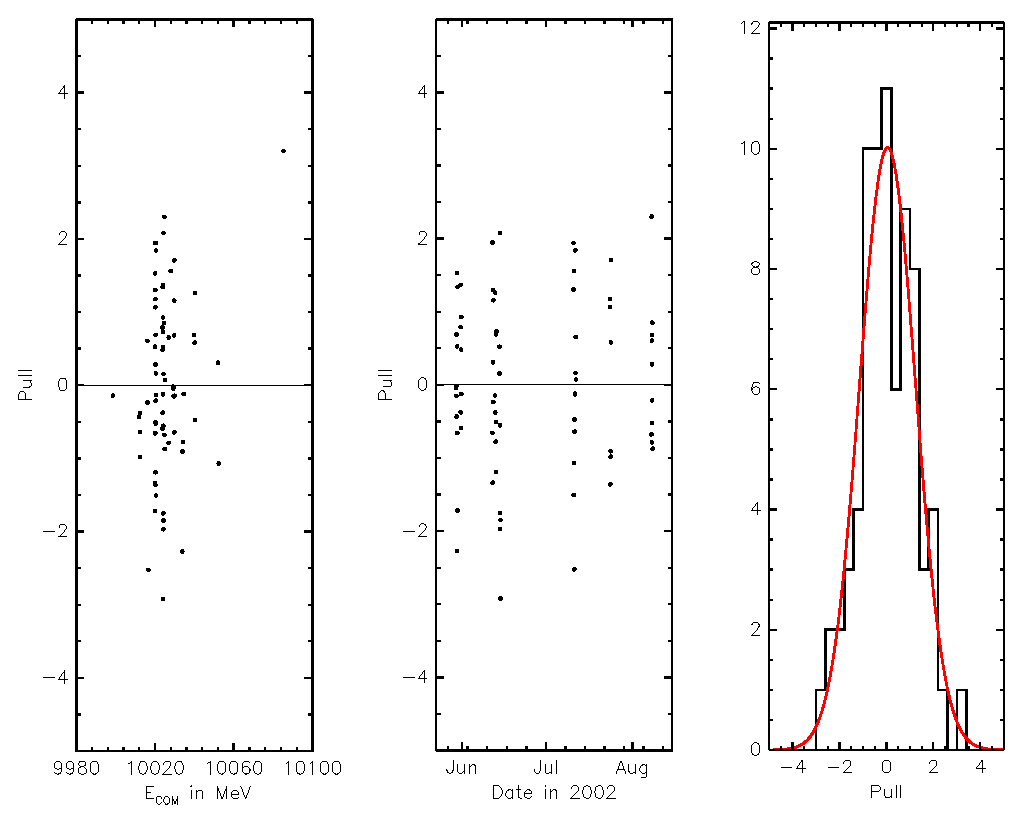
\includegraphics[width=0.8\linewidth]{plots/pulls2}
\end{center}

$\chi^2/N_\subs{dof}$ = 107/66 = 1.6, confidence level = 0.1\%

\end{slide:fitting}

\begin{slide:fitting}

\begin{center}
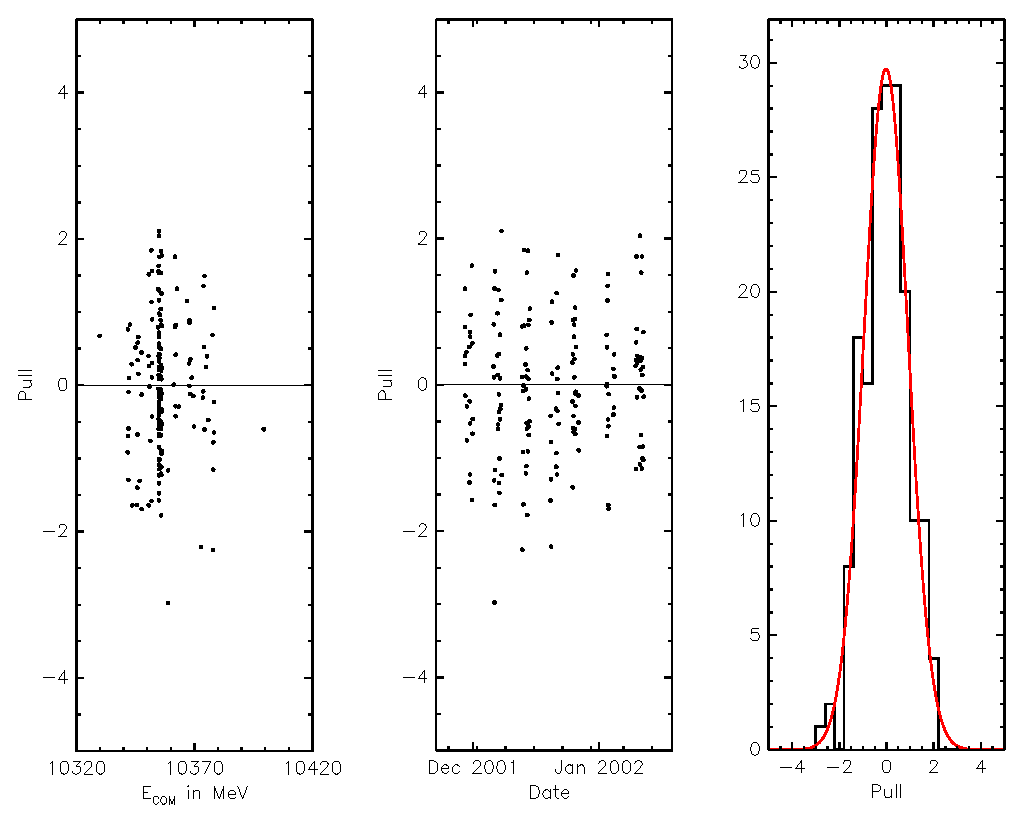
\includegraphics[width=0.8\linewidth]{plots/pulls3}
\end{center}

$\chi^2/N_\subs{dof}$ = 155/159 = 1.0, confidence level = 59\%

\end{slide:fitting}

\begin{slide:interference}

Need to consider interference between $e^+e^- \to \Upsilon \to q\bar{q}$ and $e^+e^- \to q\bar{q}$

\vfill
Resonance and continuum {\it amplitudes} add, not cross-sections \hfill ($\sigma \propto {\mathcal A}^2$)

\vfill
Phase difference cycles through resonance: destructive interference below resonance, \mbox{constructive} above

\vfill
\begin{center}
\begin{tabular}{p{0.45\linewidth} p{0.45\linewidth}}
\begin{minipage}{\linewidth}
\vspace{1.5 cm}
{\color{red} red:} no interference

{\color{blue} blue:} exaggerated interference

\vspace{0.25 cm}
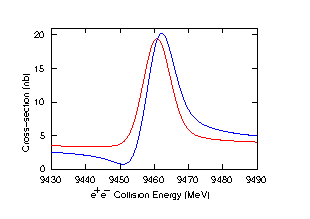
\includegraphics[width=\linewidth]{plots/interference}
\end{minipage} &
\begin{minipage}{\linewidth}
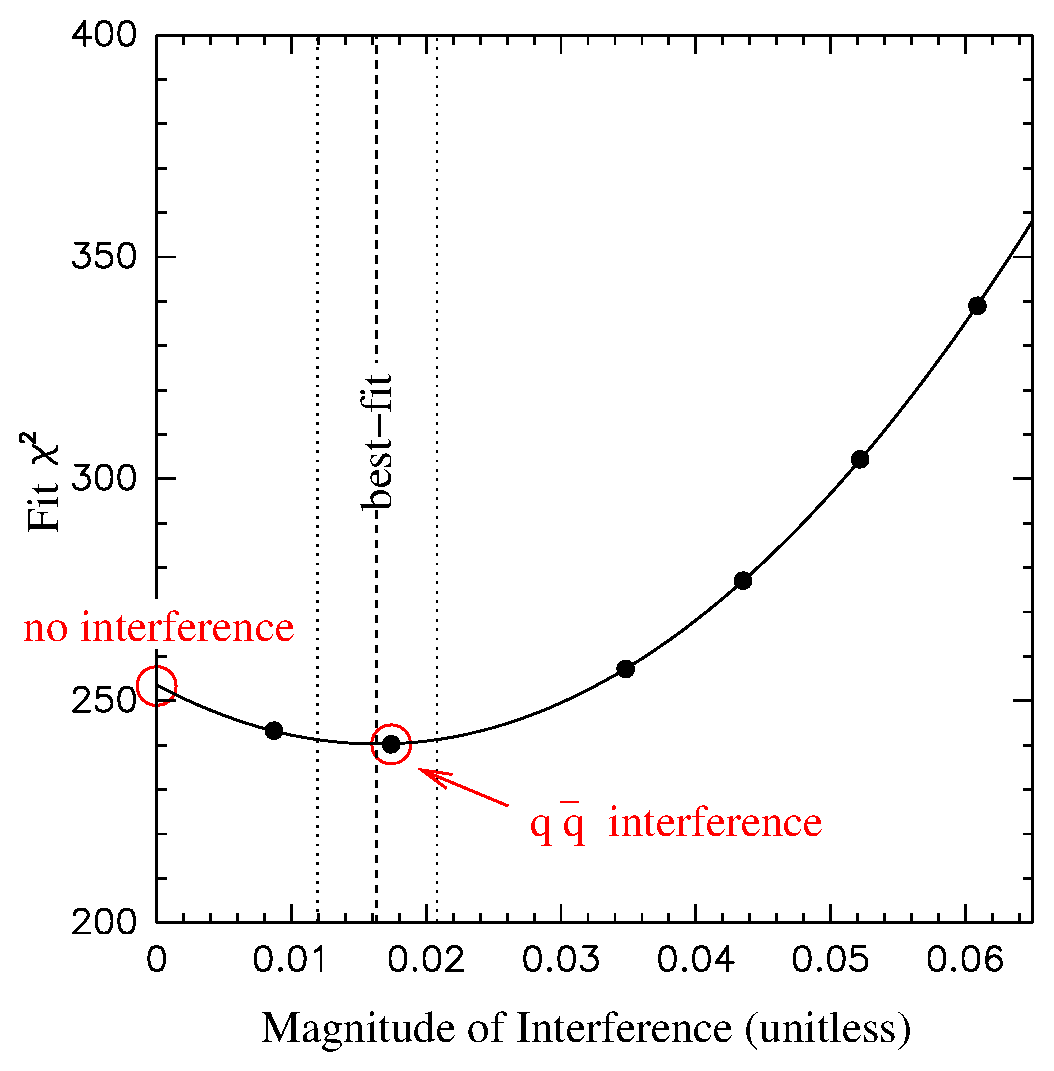
\includegraphics[width=\linewidth]{plots/simpleintfit}
\end{minipage}
\end{tabular}
\end{center}

\end{slide:interference}

\begin{slide:interference}

Does $q\bar{q} \to$ hadronic interfere with $ggg \to$ hadronic?

\vfill
Exclusive final states known to interfere (``hadronic'' = $\pi^+\pi^-$, $K^+K^-$)

\vfill
Do they interfere inclusively (sum over all final states)? or do phases wash out?

\vfill
Our fits provide first constraints, as a function of $q\bar{q} - ggg$ phase difference

\vfill
\begin{center}
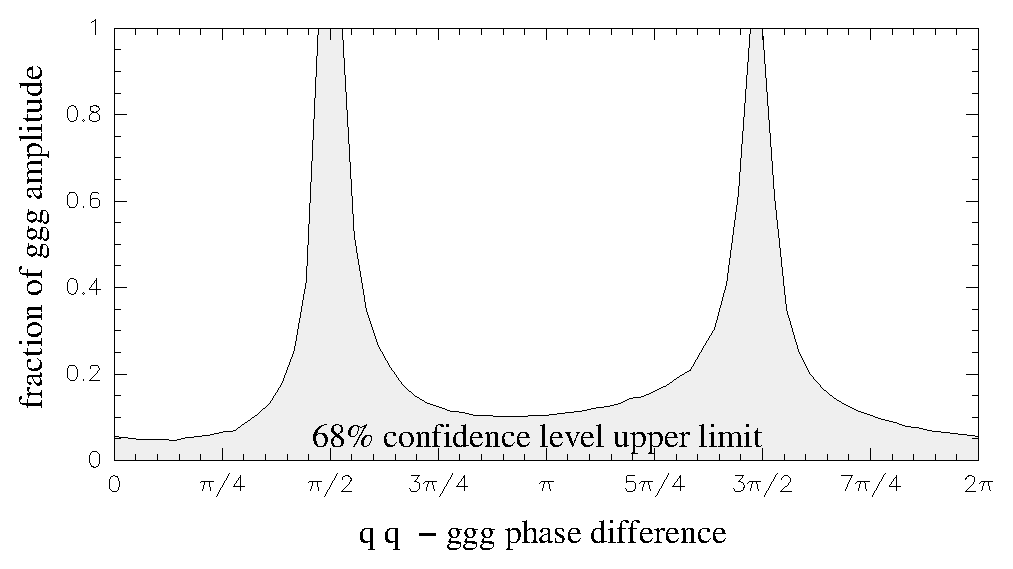
\includegraphics[width=0.65\linewidth]{plots/intconstraint}
\end{center}

\vfill
We assume no \qqbar/$ggg$ interference in our \gee\ fits

\end{slide:interference}

\begin{slide:conclusions}

\begin{center}
\begin{minipage}{0.9\linewidth}
Summary of All Uncertainties \hfill {\color{blue} $^*$Common to all resonances}
\end{minipage}
\end{center}

\begin{center}
  \renewcommand{\arraystretch}{1.3}
  \begin{tabular}{l c c c}
    \hline\hline Contribution to \gee & \hspace{0.5 cm}\us\hspace{0.5 cm} & \hspace{0.5 cm}\uss\hspace{0.5 cm} & \hspace{0.5 cm}\usss\hspace{0.5 cm} \\\hline
    Correction for leptonic modes        	   & 0.2\%  & 0.2\%  & 0.3\%  \\
    {\color{blue} Hadronic efficiency$^*$} & {\color{blue} 0.5\%}  & {\color{blue} 0.5\%}  & {\color{blue} 0.5\%}  \\
    $Xe^+e^-$, $X\mu^+\mu^-$ correction  	   & 0      & 0.15\% & 0.13\% \\
    {\color{blue} Overall luminosity scale$^*$} & {\color{blue} 1.3\%}  & {\color{blue} 1.3\%}  & {\color{blue} 1.3\%}  \\
    Bhabha/$\gamma\gamma$ inconsistency  	   & 0.4\%  & 0.4\%  & 0.4\%  \\
    Beam energy measurement drift \hspace{0.5 cm}  & 0.2\%  & 0.2\%  & 0.2\%  \\
    Fit function shape                   	   & 0.1\%  & 0.1\%  & 0.1\%  \\
    $\chi^2$ inconsistency               	   & 0.2\%  & 0.6\%  & 0      \\\hline
    Total systematic uncertainty         	   & {\color{red} 1.5\%}  & {\color{red} 1.6\%}  & {\color{red} 1.5\%}  \\
    Statistical uncertainty              	   & 0.3\%  & 0.7\%  & 1.0\%  \\\hline
    Total                                	   & {\color{red} 1.5\%}  & {\color{red} 1.8\%}  & {\color{red} 1.8\%}  \\\hline\hline
  \end{tabular}
\end{center}

\end{slide:conclusions}

\begin{slide:conclusions}

\begin{center}
\begin{minipage}{0.9\linewidth}
Results!
\end{minipage}
\end{center}

\begin{center}
\renewcommand{\arraystretch}{1.8}
\begin{tabular}{c c c c}
  \boldmath $\Gamma_{ee}(1S)$ & \mbox{\hspace{0.25 cm}} = \mbox{\hspace{0.25 cm}} & 1.354 $\pm$ 0.004 $\pm$ 0.020 keV & \mbox{\hspace{0.5 cm}} 1.5\% \mbox{\hspace{0.5 cm}} \\
  \boldmath $\Gamma_{ee}(2S)$ & = & 0.619 $\pm$ 0.004 $\pm$ 0.010 keV & 1.8\% \\
  \boldmath $\Gamma_{ee}(3S)$ & = & 0.446 $\pm$ 0.004 $\pm$ 0.007 keV & 1.8\% \\\hline

  \boldmath $\Gamma_{ee}(2S)/\Gamma_{ee}(1S)$ & = & 0.457 $\pm$ 0.004 $\pm$ 0.004 keV & 1.2\% \\
  \boldmath $\Gamma_{ee}(3S)/\Gamma_{ee}(1S)$ & = & 0.329 $\pm$ 0.003 $\pm$ 0.003 keV & 1.3\% \\
  \boldmath $\Gamma_{ee}(3S)/\Gamma_{ee}(2S)$ & = & 0.720 $\pm$ 0.009 $\pm$ 0.007 keV & 1.6\% \\\hline

  \boldmath $\Gamma(1S)$ & = & 54.4 $\pm$ 0.2 $\pm$ 0.8 $\pm$ 1.6 keV & 3.3\% \\
  \boldmath $\Gamma(2S)$ & = & 30.5 $\pm$ 0.2 $\pm$ 0.5 $\pm$ 1.3 keV & 4.6\% \\
  \boldmath $\Gamma(3S)$ & = & 18.6 $\pm$ 0.2 $\pm$ 0.3 $\pm$ $\underbrace{\mbox{0.9}}_{{\mathcal B}_{\mu\mu}}$ keV & 5.2\% \\

\end{tabular}
\end{center}

\end{slide:conclusions}

\begin{slide:conclusions}
\begin{center}
  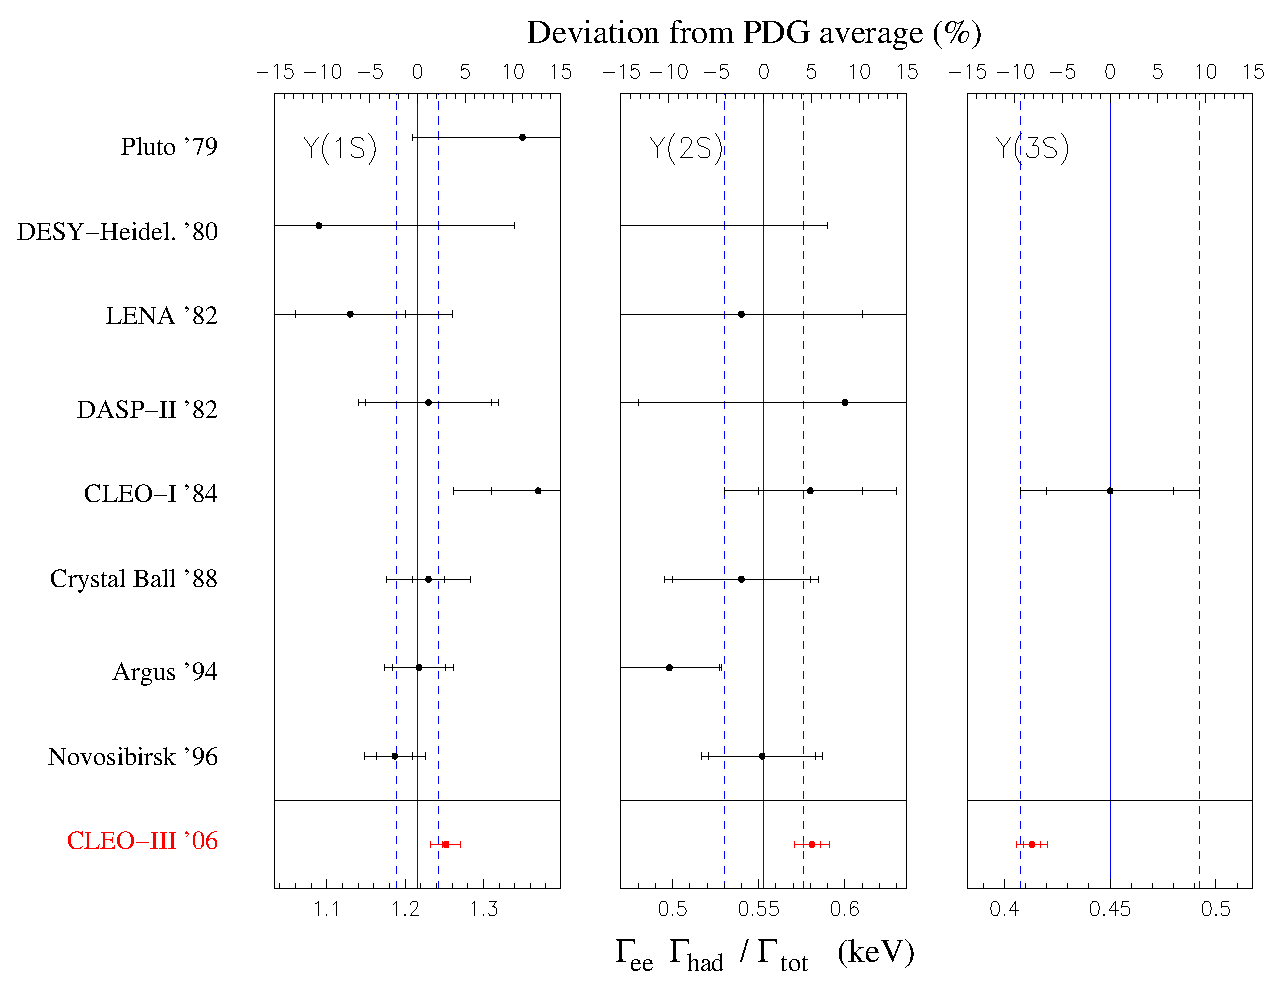
\includegraphics[width=0.85\linewidth]{plots/historyplot}
\end{center}
\end{slide:conclusions}

\begin{slide:conclusions}
\begin{itemize}

  \item Lattice QCD results are preliminary

  \item Final results will have few percent precision in $\Gamma_{ee}(nS)/\Gamma_{ee}(mS)$ and $\sim$10\% in $\Gamma_{ee}(nS)$

\end{itemize}

\vfill
\begin{center}
  \includegraphics[width=0.8\linewidth]{plots/latticespacingagain}
\end{center}

\vfill
\Large
\hfill A.~Gray {\it et al.} [HPQCD Collaboration], Phys.\ Rev.\ D {\bf 72}, 094507 (2005) \hspace{1.3 cm}

\end{slide:conclusions}

\end{document}
